\documentclass{article}
\usepackage{bookmark}

\usepackage[utf8]{inputenc}
\usepackage[brazil]{babel}  % Define o idioma para português do Brasil
\usepackage{csquotes}       % Para lidar com aspas de maneira apropriada com babel
%\usepackage{ragged2e}       % Pacote para justificação

\usepackage{amsmath}
\usepackage{xcolor}
\usepackage{listings}
% Configuração do estilo de código
\lstset{
  language=C,
  %basicstyle=\ttfamily\footnotesize,
  keywordstyle=\color{blue},
  commentstyle=\color{gray},
  stringstyle=\color{red},
  breaklines=true,
  frame=single,
  numbers=left,
  numberstyle=\tiny,
  numbersep=5pt,
  showstringspaces=false,
}


\usepackage{graphicx}       % Pacote para inserção de imagens

\usepackage{hyperref}       % Pacote para links clicáveis
\hypersetup{
    colorlinks=true,
    linkcolor=blue,
    urlcolor=blue,
}

\usepackage{enumitem}       % Pacote para personalização de listas

\usepackage{geometry}       % Pacote para ajustar margens

\geometry{                  % Definindo margens personalizadas (em centímetros)
  left=2.5cm,  % Margem esquerda
  right=2.5cm, % Margem direita
  top=2.5cm,   % Margem superior
  bottom=2.5cm % Margem inferior
}          

\begin{document}

\begin{titlepage}
    \centering
    % Cabeçalho personalizado
    
\includegraphics[width=0.3\textwidth]{./Images/Logo UFLA - Colorida chapada.png}

    \vspace*{2cm} % Espaçamento vertical antes do cabeçalho
    \Large
    Universidade Federal de Lavras\\
    PPGCC\\
    PCC508 – Sistemas Operacionais\\
    
    \vspace{2cm} % Espaço entre o cabeçalho e o título
    \huge % Define o tamanho da fonte do título
    \textbf{Tópico 3 Lista Adicional 1}
    
    \vfill % Adiciona um espaçamento flexível antes do rodapé (opcional)
    
    % Opcionalmente, você pode incluir seu nome e a data aqui
    \large
    Douglas Aquino T. Mendes\\
    \today % Insere a data atual
\end{titlepage}

\tableofcontents
\newpage

\section{Introdução}
Este documento tem como objetivo apresentar o desenvolvimento de atividades adicionais para a disciplina de Sistemas Operacionais, focando na implementação de códigos em linguagem C. Cada atividade foi elaborada com a intenção de abordar conceitos relacionados ao funcionamento de sistemas operacionais, incluindo gerenciamento de processos, gerenciamento de memória, e comunicação entre processos. Serão apresentados os códigos desenvolvidos, seguidos de uma explicação sobre sua lógica de funcionamento e objetivos.

\subsection{Bibliotecas}
Neste trabalho, diversas bibliotecas foram empregadas para facilitar o desenvolvimento dos códigos em linguagem C. Abaixo estão as principais bibliotecas utilizadas, juntamente com suas respectivas funcionalidades:

\begin{itemize}
    \item \texttt{stdio.h}: Fornece funções para entrada e saída padrão, como \texttt{printf()} e \texttt{scanf()}, permitindo interações com o usuário através do console.
    
    \item \texttt{stdlib.h}: Contém funções para manipulação de memória dinâmica (\texttt{malloc()}, \texttt{free()}) e outras utilidades gerais, essenciais para o gerenciamento de recursos.
    
    \item \texttt{string.h}: Oferece funções para manipulação de strings, como \texttt{strlen()}, \texttt{strcpy()} e \texttt{strcat()}, facilitando o processamento de dados textuais.
    
    \item \texttt{dirent.h}: Utilizada para manipulação de diretórios, permitindo listar arquivos e acessar informações sobre diretórios no sistema de arquivos.
    
    \item \texttt{ctype.h}: Fornece funções para testes de caracteres e conversões, como \texttt{isdigit()} e \texttt{tolower()}, que são úteis para operações relacionadas a caracteres.
    
    \item \texttt{unistd.h}: Contém declarações para chamadas de sistema POSIX, permitindo operações de baixo nível, como leitura e gravação em arquivos, além de manipulação de processos.
    
    \item \texttt{sys/types.h}: Define tipos de dados utilizados em chamadas de sistema, incluindo definições para identificadores de processos e modos de arquivos.
    
    \item \texttt{sys/wait.h}: Oferece macros para controle de processos, permitindo que um processo pai espere a terminação de processos filhos.
    
    \item \texttt{pthread.h}: Utilizada para programação concorrente, permitindo a criação e manipulação de threads, essencial para o desenvolvimento de aplicações que requerem multitarefa.
    
    \item \texttt{sys/mman.h}: Contém funções para manipulação de memória, como mapeamento de arquivos e alocação de memória compartilhada.
    
    \item \texttt{semaphore.h}: Fornece definições e funções para o uso de semáforos, que são utilizados para controlar o acesso a recursos compartilhados em ambientes concorrentes.
    
    \item \texttt{fcntl.h}: Utilizada para controle de arquivos, permitindo operações como bloqueio de arquivos e manipulação de descritores de arquivos.
    
    \item \texttt{sys/stat.h}: Define a estrutura de dados e funções para obter informações sobre arquivos, como tipo, permissões e tamanhos.
\end{itemize}

\section{Atividade 1}
\subsection{Descrição}
O diretório /proc/PID apresenta vários arquivos com informações sobre os processos em execução na máquina. Em especial, o arquivo status apresenta informações de estado sobre um processo. Fazer um programa que receba uma string na entrada e apresente as informações do arquivo status de todos os processos que tenham essa string como substring do nome do processo.
\subsection{Código}
\lstinputlisting[language=C]{Codes/atv1.c}
\subsection{Testes e Resultados}
Como teste, foi dado a string "bash" como entrada como é ilustrado na figura \ref{fig:atv1_entrada}, e alguns dos resultados podem ser visualizados nas figuras \ref{fig:atv1_result1} e \ref{fig:atv1_result2}.

\begin{figure}[ht]
    \centering
    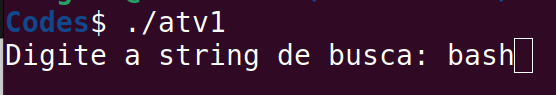
\includegraphics[width=0.5\textwidth]{./Images/atv1_entrada.png}
    \caption{String de entrada}
    \label{fig:atv1_entrada}
\end{figure}

\begin{figure}[ht]
    \centering
    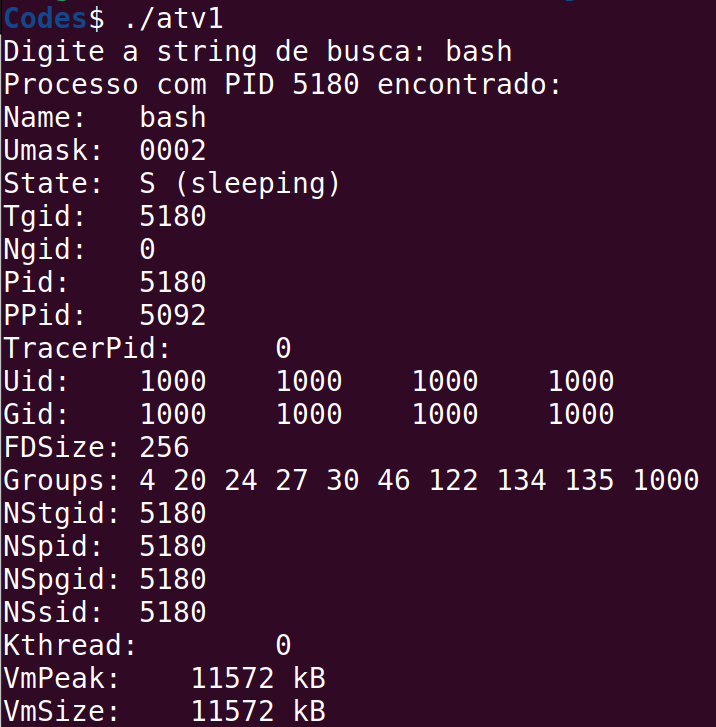
\includegraphics[width=0.5\textwidth]{./Images/atv1_result1.png}
    \caption{Resultado 1 da execução do programa}
    \label{fig:atv1_result1}
\end{figure}

\begin{figure}[ht]
    \centering
    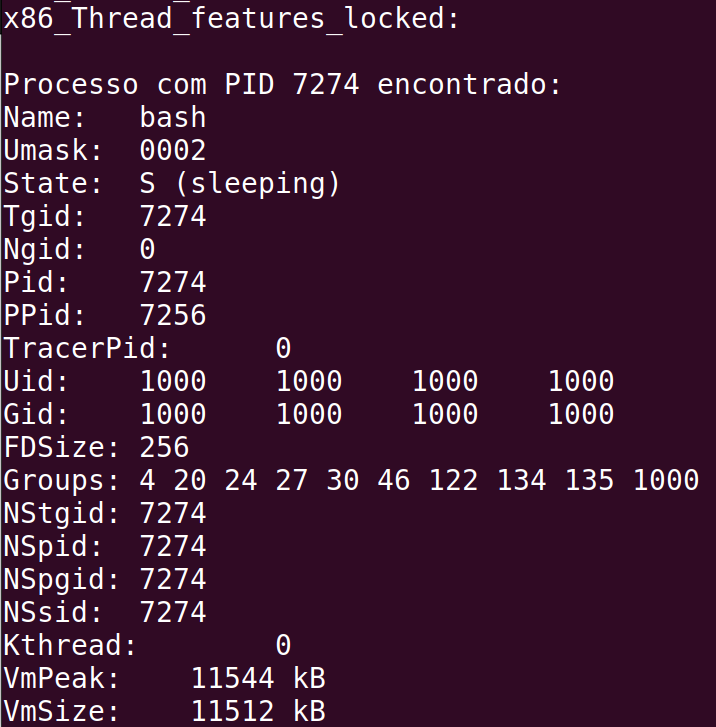
\includegraphics[width=0.5\textwidth]{./Images/atv1_result2.png}
    \caption{Resultado 2 da execução do programa}
    \label{fig:atv1_result2}
\end{figure}
\newpage

\section{Atividade 2}
\subsection{Descrição}
Um shell no Unix é resposável por receber comandos do usuário e executá-los, em linha de comando. Criar um mini-shell que permita o usuário executar comandos que são executáveis no Linux. Para isso, use as chamadas de sistema fork/execve. Permita também o usuário listar os arquivos do diretório atual com ls, que nesse caso será implementado como comando interno.
\subsection{Código}
\lstinputlisting[language=C]{Codes/atv2.c}
\subsection{Testes e Resultados}
Para teste da atividade 2, primeiramente tentamos o comando ls que lista o diretório atual, como é possível observar na figura \ref{fig:atv2_result}, o diretório apenas possui os arquivos das atividades. Infelizmente o programa desenvolvido não colore os arquivos de acordo com sua propriedade, com isto, fica difícil diferenciar os arquivos de texto, de executáveis e pastas. Continuando os testes, foi criado um novo diretório chamado "teste" e novamente ls para mostrar que agora há um novo diretório. Como dificuldade, enquanto estava desenvolvendo o programa, por conta de um erro de lógica, o argumento não era passado corretamente, e acabei criando uma pasta com alguma referencia de lixo de memória a qual não conseguia excluir, como pode ser visto na figura \ref{fig:atv2_err}

\begin{figure}[ht]
    \centering
    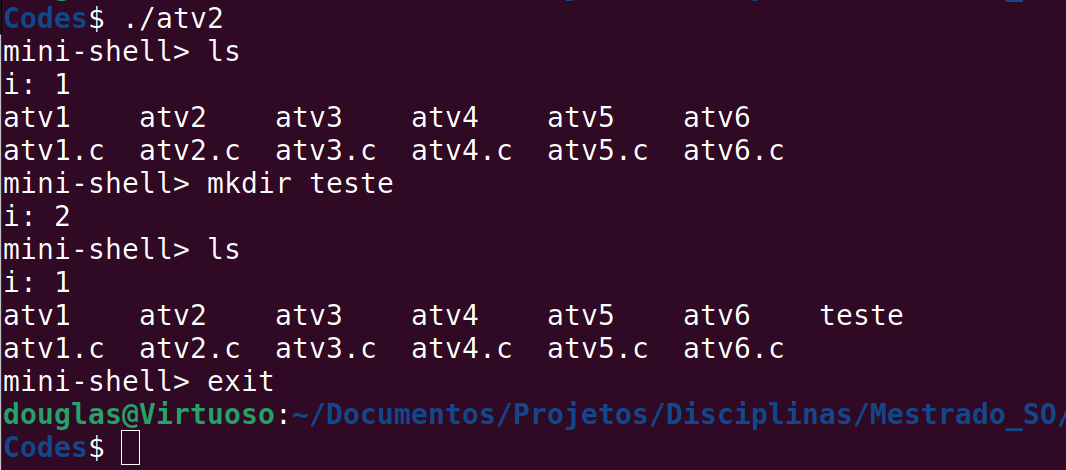
\includegraphics[width=0.5\textwidth]{./Images/atv2_result.png}
    \caption{Resultado da execução do programa 2}
    \label{fig:atv2_result}
\end{figure}

\begin{figure}[ht]
    \centering
    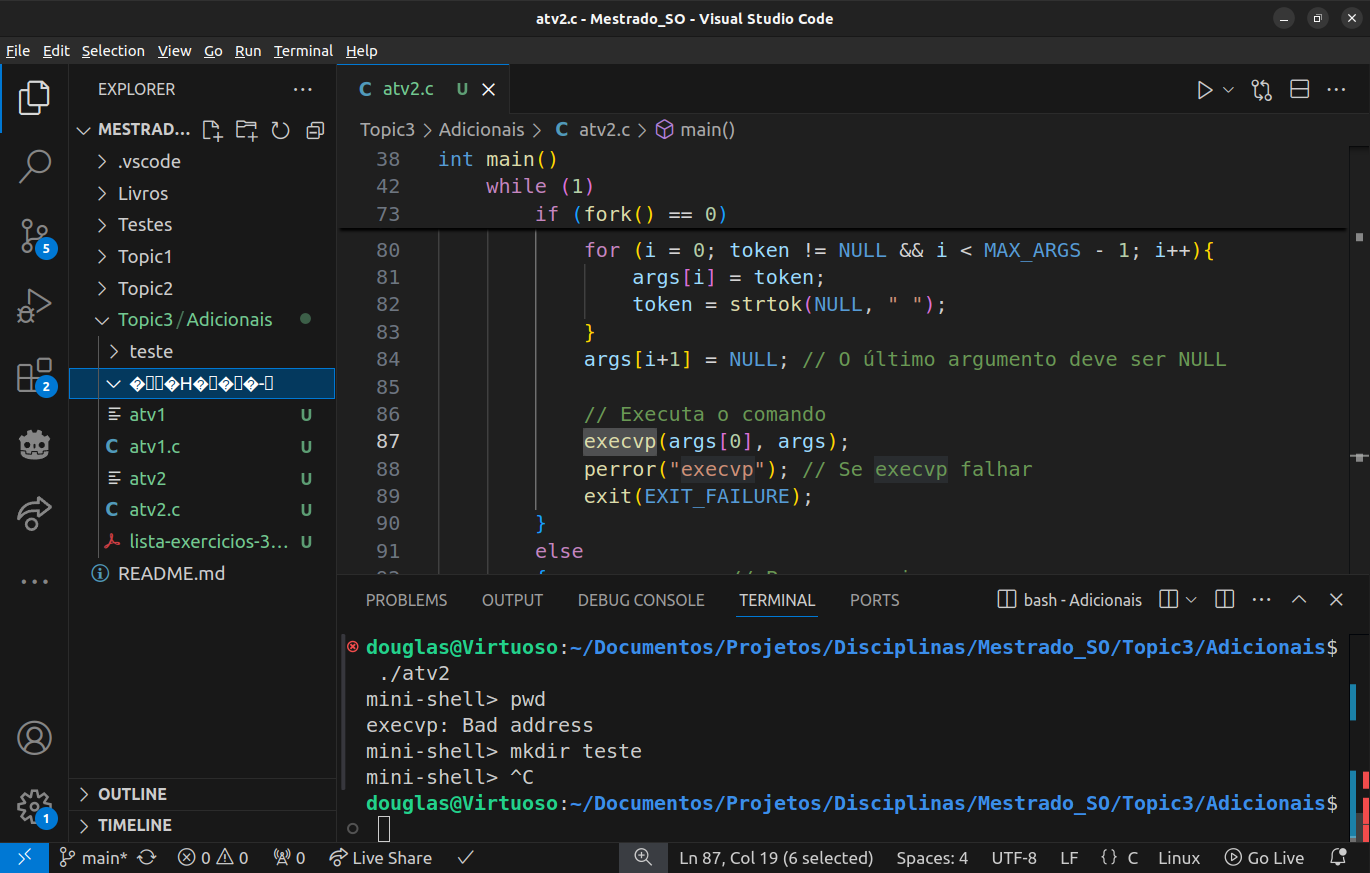
\includegraphics[width=0.8\textwidth]{./Images/atv2_err.png}
    \caption{Resultado com erro da execução do programa 2}
    \label{fig:atv2_err}
\end{figure}

\section{Atividade 3}
\subsection{Descrição}
A alternância estrita é um método de obtenção de exclusão mútua com espera ocupada. Implementar 2 threads que incrementam um contador comum, onde o controle de concorrência é feito utilizando alternância estrita.
\subsection{Código}
\lstinputlisting[language=C]{Codes/atv3.c}
\subsection{Testes e Resultados}
Como é possível observar no código fonte do programa, o printf mostra no termnial qual a thread está incrementando e o valor o qual ficou o contador, com isto, temos o resultado na figura \ref{fig:atv3_result}.
\begin{figure}[ht]
    \centering
    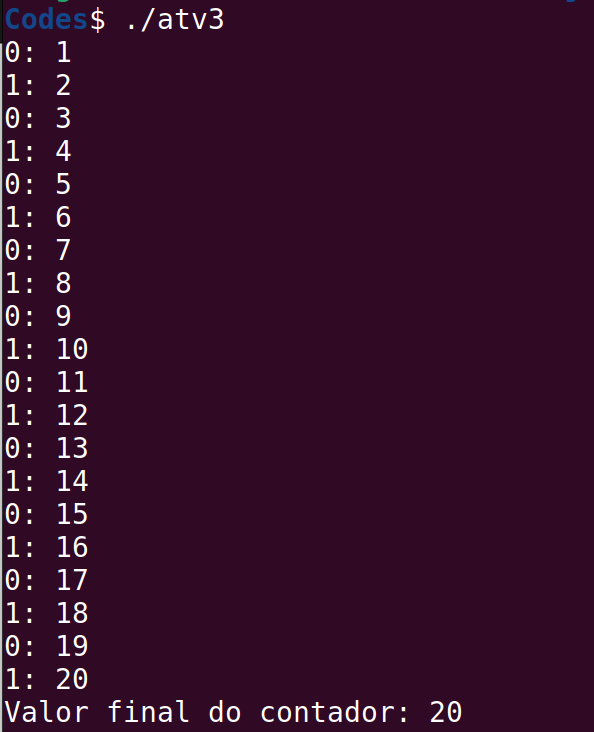
\includegraphics[width=0.6\textwidth]{./Images/atv3_result.png}
    \caption{Resultado da execução do programa 3}
    \label{fig:atv3_result}
\end{figure}

\section{Atividade 4}
\subsection{Descrição}
Implementar o problema dos filósofos glutões com semáfaforos nomeados. Cada filósofo será implementado como um processo. Para o controle de concorrência, serão utilizados uma série de semáforos nomeados. O programa deverá receber um parâmetro que é o número de filósofos a serem criados. Para criação de processos, a chamada fork deve ser utilizada.
\subsection{Código}
\lstinputlisting[language=C]{Codes/atv4.c}
\subsection{Testes e Resultados}
A figura \ref{fig:figlu} irá colaborar para compreenção e conferencia dos resultados obtidos na execução do programa, que pode ser observado nas figura \ref{fig:atv4_result} e \ref{fig:atv4_result2}.

\begin{figure}[ht]
    \centering
    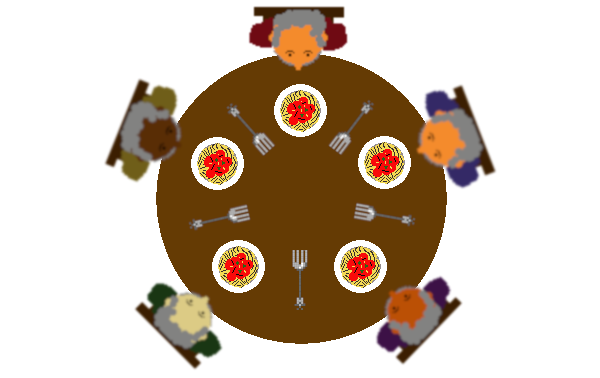
\includegraphics[width=0.4\textwidth]{./Images/figlu.png}
    \caption{Representação dos filósofos em uma mesa}
    \label{fig:figlu}
\end{figure}

\begin{figure}[ht]
    \centering
    \begin{minipage}{0.45\textwidth} % Largura da primeira imagem
        \centering
        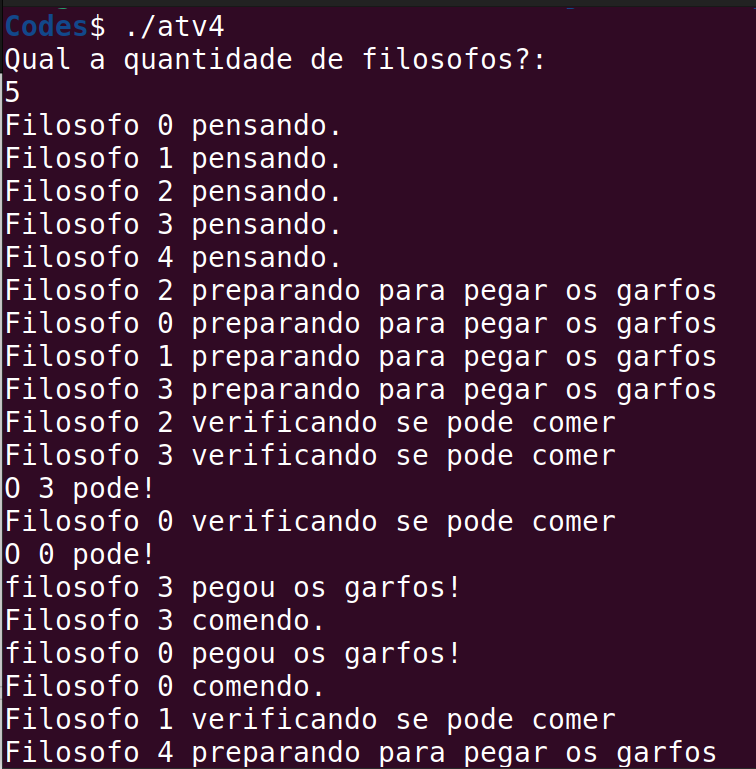
\includegraphics[width=\textwidth]{./Images/atv4_result.png} % Substitua pelo caminho da sua imagem
        \caption{Exucução do programa 4}
        \label{fig:atv4_result}
    \end{minipage} \hfill % Espaço entre as imagens
    \begin{minipage}{0.45\textwidth} % Largura da segunda imagem
        \centering
        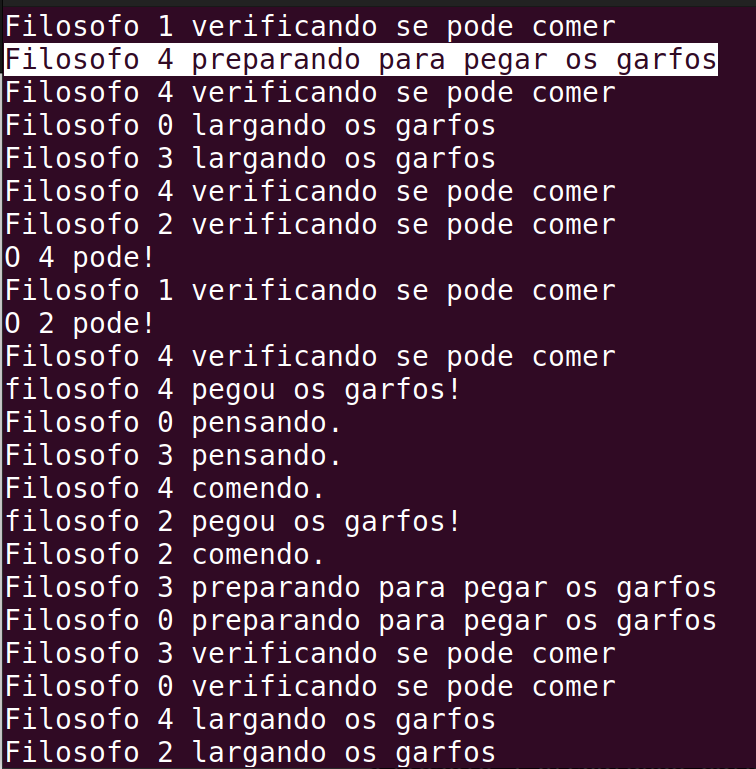
\includegraphics[width=\textwidth]{./Images/atv4_result2.png} % Substitua pelo caminho da sua imagem
        \caption{Continuação da execução do programa}
        \label{fig:atv4_result2}
    \end{minipage}
\end{figure}
\newpage

\section{Atividade 5}
\subsection{Descrição}
Implementar o problema dos produtores/consumidores utilizando threads e mutexes, juntamente com variáveis de condição.
\subsection{Código}
\lstinputlisting[language=C]{Codes/atv5.c}
\subsection{Testes e Resultados}
\begin{figure}[ht]
    \centering
    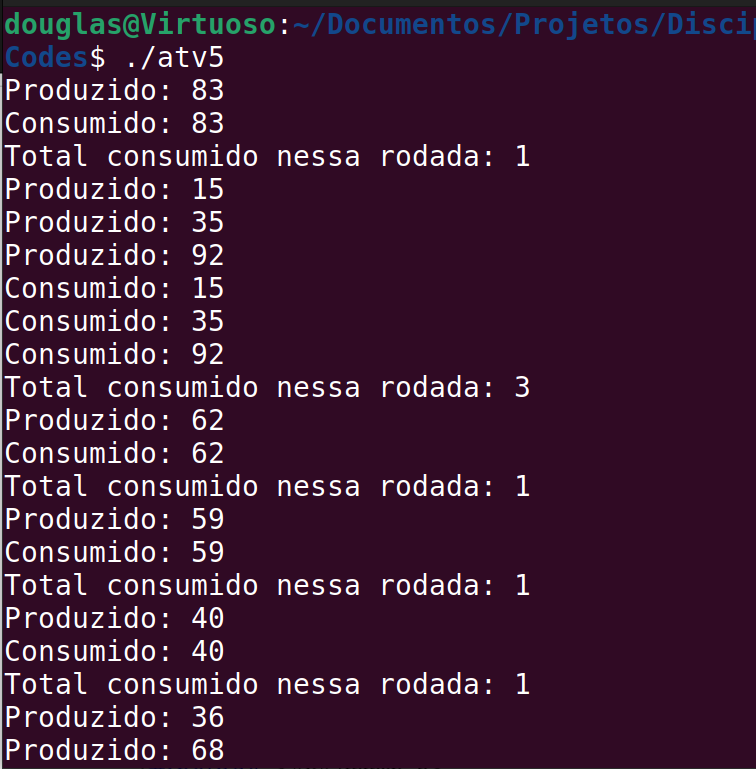
\includegraphics[width=0.6\textwidth]{./Images/atv5_result.png}
    \caption{Resultado da execução do programa 5}
    \label{fig:atv5}
\end{figure}

\section{Atividade 6}
\subsection{Descrição}
Implementar o problema dos leitores/escritores com um método de IPC a escolha.
\subsection{Código}
\lstinputlisting[language=C]{Codes/atv6.c}
\subsection{Testes e Resultados}
\begin{figure}[ht]
    \centering
    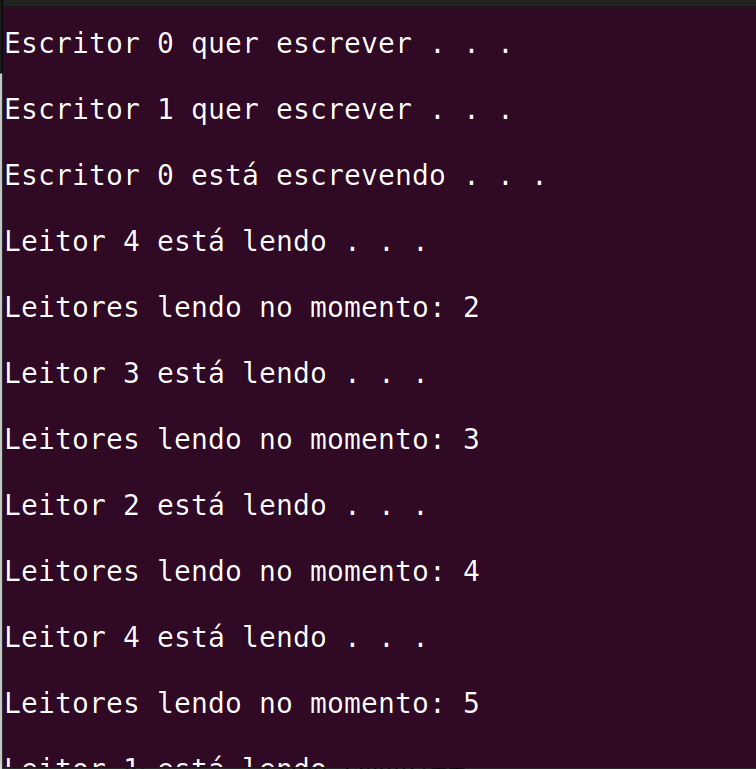
\includegraphics[width=0.6\textwidth]{./Images/atv6_result.png}
    \caption{Resultado da execução do programa 6}
    \label{fig:atv5}
\end{figure}

\end{document}